
\chapter{EXPERIMENTAL TESTS AND RESULTS. }

\section{MOILP vs MOGA}

The tests carried out considering different types of traffic load,
different values of K and different demanded quantities, try to replicate
different possible scenarios of the problem to solve. The most complex
scenarios seek to replicate real situations of traffic demands. The
experimental tests carried out show that all these scenarios can be
solved with at least one of the proposed algorithms, obtaining promising
results.

\subsection{Testing Enviroment}

The experiments were performed on a computer with an Intel Core i7
processor (2.40 GHz) and 8 GB of RAM. The engine used for the implementation
and execution of the MOILP was the IBM ILOG CPLEX Optimization Studio
Version 12.6, and the implementation and execution of the MOGA and
the GA were done with JAVA 8.

All the executed executions were executed with 3 directional network
topologies: a network of 6 nodes, the NSF topology of 14 nodes and
the Arpa-2 topology of 21 nodes which can be observed in Figures \ref{topology_6nodes_figure},
\ref{topology_nsf_figure} y \ref{topology_arpa-2_figure}. The number
of FSs in the optical links has been considered without limit given
that the problem is of the static type corresponding to a planning.

\begin{figure}
\begin{centering}
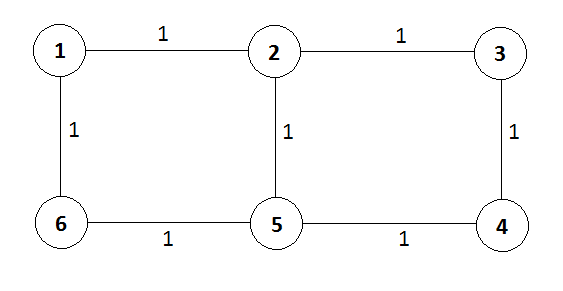
\includegraphics{G:/Genetico/LIBRO_TESIS/04.ListaFiguras/6nodos}
\par\end{centering}
\caption{6 node network topology.}
\label{topology_6nodes_figure}
\end{figure}

\begin{figure}
\begin{centering}
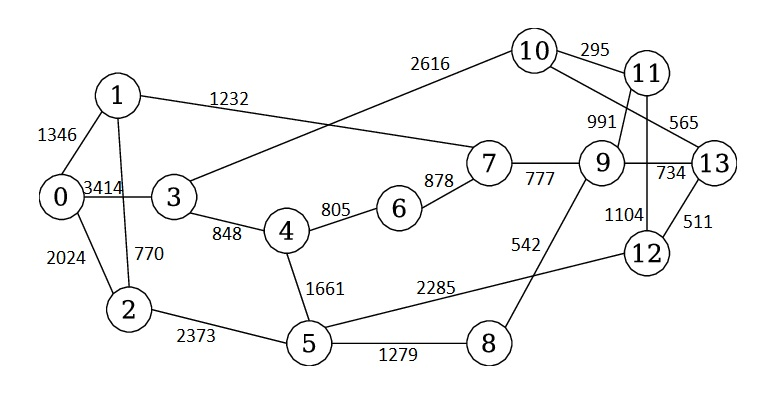
\includegraphics[scale=0.6]{G:/Genetico/LIBRO_TESIS/04.ListaFiguras/nsf_topology}
\par\end{centering}
\caption{Topology of NSF network of 14 nodes with distance in kilometers}
\label{topology_nsf_figure}
\end{figure}

\begin{figure}
\begin{centering}
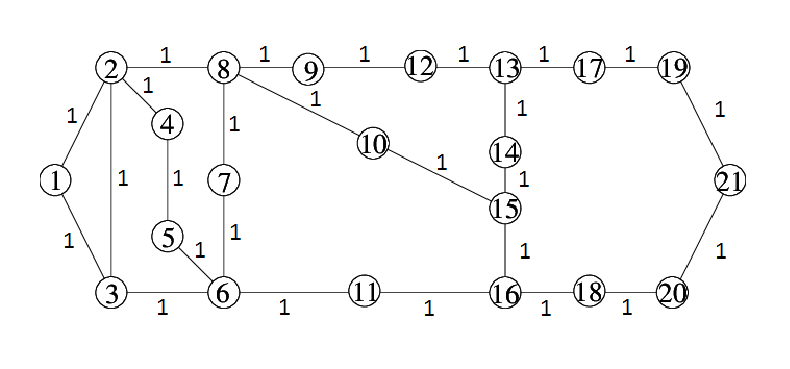
\includegraphics{G:/Genetico/LIBRO_TESIS/04.ListaFiguras/arpa-2}
\par\end{centering}
\caption{21-node Arpa-2 network topology}
\label{topology_arpa-2_figure}
\end{figure}

The traffic loads used were of the all-to-all type, that is, each
node of the network makes a transfer request to all other nodes in
the network. In addition, said traffic loads were divided into two
types: uniform traffic load and random traffic load. In the first,
all the demands request the same amount of FS, the requested quantities
were: 50, 100, 150 and 200 FS. For the random loads, they were also
divided into 4 categories but these quantities were used as the maximum
quantity, that is, for the category of 50 FS, for each demand a random
value between 1 and 50 was generated as requested amount of FS; for
the category of 100, for each demand a random value between 1 and
100 was generated as requested quantity of FS; for the category of
150, for each demand a random value between 1 and 150 was generated
as requested quantity of FS; and finally for the category of 200 for
each demand, a random value between 1 and 200 was generated as requested
quantity of FS.

Another variant that was taken into account for the execution of the
tests was the quantity of precalculated shorter routes, that is, the
value of k. The executions of the MOGA and the GA were made with the
following values of k = 1, 2, 3, 4, 5, 6 and 7, except for the topology
of 6 nodes since in this topology there are up to 3 paths for each
pair of nodes The MOILP was executed with the following values of
k: for the topology of 6 nodes, k = 1, 2 and 3 were used with a time
limit of 2 hours; for the NSF topology a time limit of 4 hours was
defined and results were obtained with k = 1, 2, 3, 4 and 5, except
for the demand scenarios of 200 FS in which only results were obtained
up to k = 4; and for the ARPA-2 topology, a time limit of 4 hours
was also defined and results were obtained only for k = 1. The limitation
in the executions of the MOILP is given by the size of the topologies,
since the ILP implementations are not Generally scalable.

For the executions of the MOGA, the values shown in Table \ref{tabla:moga_params}
were used as evolutionary parameters.

Since the MOGA and the GA are stochastic algorithms, each execution
can present different results. Taking into account this factor, with
the MOGA several executions were carried out for each proposed scenario.
The number of executions per scenario is defined by the parameter
Quantity of independent runs in Table \ref{tabla:moga_params}.

The final results of the MOGA are the average values obtained from
all the executions of each scenario, that is, from 30 independent
runs performed for a scenario, the values of the objective functions
were averaged and said values are those presented in the results.

 \begin{table}[!t] 	
	\centering 	
		\caption{Parameters used for the execution of the MOGA.} 	
		\begin{tabular}{*{2}{|c}|} 		
			\hline 		
			\scriptsize {\textbf{Parameter}} & \scriptsize {\textbf{Value}} \\ 		
			\hline 		
			\scriptsize {Size of the population} & \scriptsize {100} \\ 		
			\hline 		
			\scriptsize {Probability of mutation} & \scriptsize {2\%} \\ 		
			\hline 		
			\scriptsize {Stop criterion} & \scriptsize {5 minutos de ejecuci�n} \\ 		
			\hline 		
			\scriptsize {Number of independent runs} & \scriptsize {30} \\ 		
			\hline 	
		\end{tabular} 	
		\label{tabla:moga_params} 
\end{table} 

\begin{table}[!t] 	
	\centering 	
	\caption{Scenarios of executions.} 	
	\begin{tabular}{ | c | c | >{\centering}m{4,7cm} | c |} 		
		\hline 		
		\scriptsize {\textbf{Topology}} & 
		\scriptsize {\textbf{K}}  & 
		\scriptsize {\textbf{Load}}  & 
		\scriptsize {\textbf{Time}}\\ 		
		\hline 		
		\scriptsize {6-nodes} & \scriptsize {1, 2, 3} & 
		\scriptsize{Uniform 50, 100, 150, 200 Aleatoria: 1-50, 1-100, 1-150, 1-200} & 
		\scriptsize{MOILP: 2 hs, MOGA: 5$\cdot$30 = 150 minutes} \\ 		
		\hline 		
		\scriptsize {NSF} & \scriptsize {1, 2, 3, 4, 5, 6} & 
		\scriptsize{Uniform 50, 100, 150, 200 Aleatoria: 1-50, 1-100, 1-150, 1-200} & 
		\scriptsize{MOILP: 4 hs, MOGA: 5$\cdot$30 = 150 minutes} \\ 		
		\hline 		
		\scriptsize {ARPA-2} & \scriptsize {1, 2, 3, 4, 5, 6} & 
		\scriptsize{Uniform 50, 100, 150, 200 Aleatoria: 1-50, 1-100, 1-150, 1-200} & 
		\scriptsize{MOILP: 4 hs, MOGA: 5$\cdot$30 = 150 minutes} \\ 		
		\hline 	
	\end{tabular} 	
	\label{tabla:escenarios} 
\end{table} 

In Table \ref{tabla:escenarios}, we can see a summary of the executed
scenarios. The topologies used are shown, the values of K for each
topology, the traffic loads (which were divided into uniform load
and random load), and the execution time which, in the case of MOILP,
represent the time limit of defined execution, and in the case of
the MOGA, they represent the total execution time, since for each
independent execution 5 minutes were defined as stopping criteria
and 30 scenarios were performed for each scenario.

Basically, given a scenario consisting of a topology, a number of
routes and traffic load, we proceed to:

\begin{enumerate}     
	\item Calculate a MOILP solution 
	\item Calculate 30 MOGA solutions 
	\item Calculate average values of the 30 MOGA solutions of the objective and Fitness functions 
	\item Calculate 30 GA solutions 
	\item Calculate average values of the 30 GA solutions of the objective functions and Fitness 
	\item Perform analysis of the solutions
\end{enumerate} 

Based on these steps, the following experimental results are presented.

\subsection{Uniform Load Results: MOILP vs MOGA}

In this section we analyze all the results of the objective and fitness
functions, MOILP and MOGA. 

The Figures \ref{6nodos_ilp_fitness}, \ref{6nodos_ilp_fs}, \ref{6nodos_ilp_distance}
and \ref{6nodos_ilp_cost} show the values obtained by the Fitness
MOILP, maximum FS, total distance and total cost, repectively, for
the topology of 6 nodes. The value shown in the vertical axis is the
value of the objective function, and results were obtained up to k
= 3, since with a topology of 6 nodes there are no more than 3 possible
paths for each pair of nodes. When analyzing the Figure \ref{6nodos_ilp_fitness}
it can be seen that having 2 possible ways the fitness value improves,
that is, with k = 2 a great improvement was obtained compared to k
= 1.

It can be observed that by having two possible routes to satisfy the
demands, a second route was used in one or several demands, which
increased the value of the total distance traveled as shown in Figure
\ref{6nodos_ilp_distance}, since the first route is the shortest.
But using a longer route produced a better use of the available spectrum,
since for k = 2, in Figure \ref{6nodos_ilp_fs} a decrease in the
maximum FS used is observed.

Another observation that can be made about these results is that the
greatest improvement was obtained from k = 1 to k = 2, since with
k = 3 practically the fitness value is maintained.

With the results mentioned above, the proposed MOILP implementation
is validated. The same behavior is observed for the topology NSF-14
in the Figures \ref{nsf-14_ilp_fitness}, \ref{nsf-14_ilp_fs}, \ref{nsf-14_ilp_distance}
and \ref{nsf-14_ilp_cost} obtaining results up to k = 5 except for
the 200 FS load that could only be calculated with solutions up to
k = 4. For the ARPA-2 topology, only solutions with k = 1 could be
calculated.

The Figures \ref{6nodos_moga1_fitness}, \ref{6nodos_moga1_fs}, \ref{6nodos_moga1_distance}
and \ref{6nodos_moga1_cost} show the values of fitness, maximum FS,
total distance, and total cost, respectively, obtained by the MOGA
for the topology of 6 nodes. It can be observed that it manages to
obtain practically the same results as the MOILP with values close
to the optimum.

The results obtained by the MOGA for the fitness and the objective
functions of the topology NSF-14, are shown in the Figures \ref{nsf-14_moga1_fitness},
\ref{nsf-14_moga1_fs}, \ref{nsf-14_moga1_distance} and \ref{nsf-14_moga1_cost}.
It can also be observed that the most significant improvement occurs
with k = 2, from k = 3 almost no changes are seen in the results and
it is converging.

Finally, the Figures \ref{arpa-2_ilp_fitness}, \ref{arpa-2_moga1_fs},
\ref{arpa-2_moga1_distance} y \ref{arpa-2_moga1_cost} show the values
of fitness and objective functions for the ARPA-2 topology obtained
by the MOGA. When observing the fitness values obtained by both implementations,
it can be verified that for all values of k in the 3 topologies, the
MOILP surpassed the results obtained by the MOGA, however, the MOGA
presents results very close to the optimum generating promising solutions.

\begin{figure}
\begin{centering}
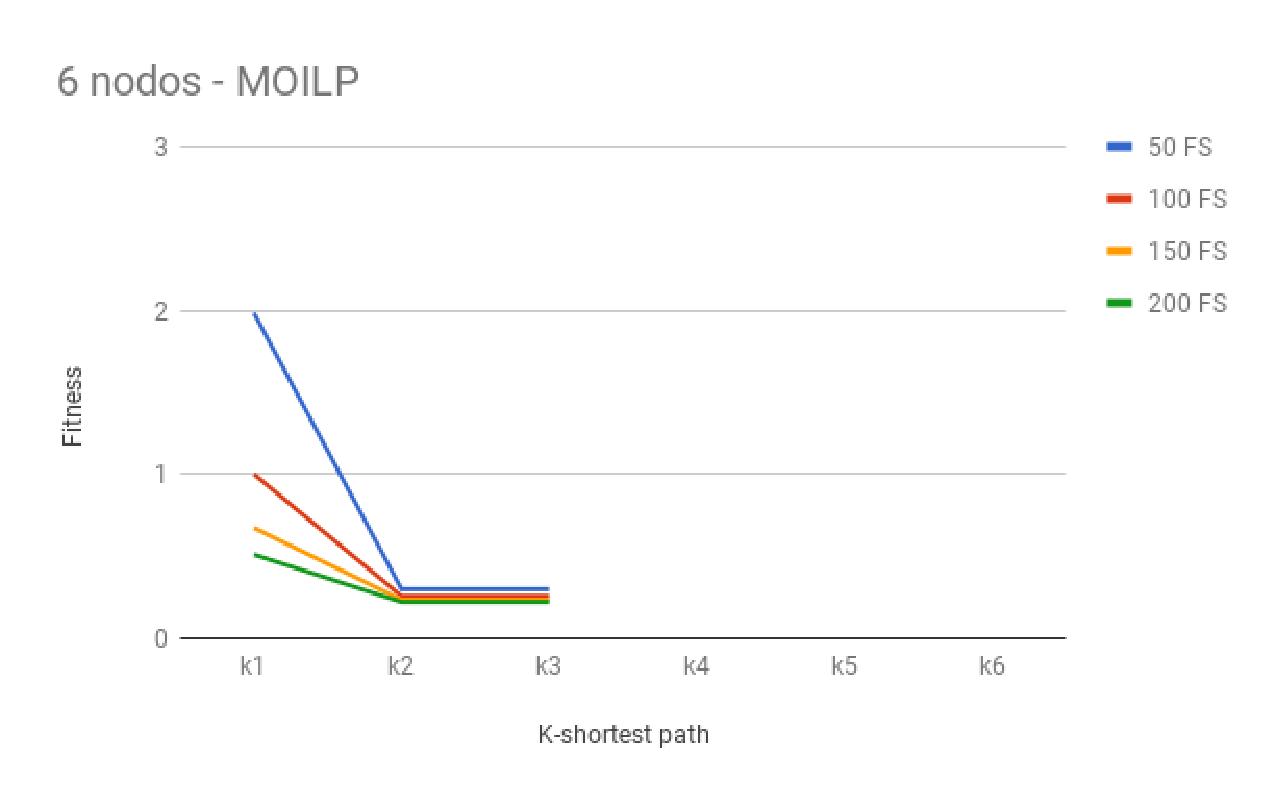
\includegraphics[scale=0.6]{G:/Genetico/LIBRO_TESIS/resulYsapy/resultados/6nodos_uniforme_ilp_fitness}
\par\end{centering}
\caption{Fitness obtained by MOILP for topology 6 nodes with uniform load.}
\label{6nodos_ilp_fitness}
\end{figure}

\begin{figure}
\begin{centering}
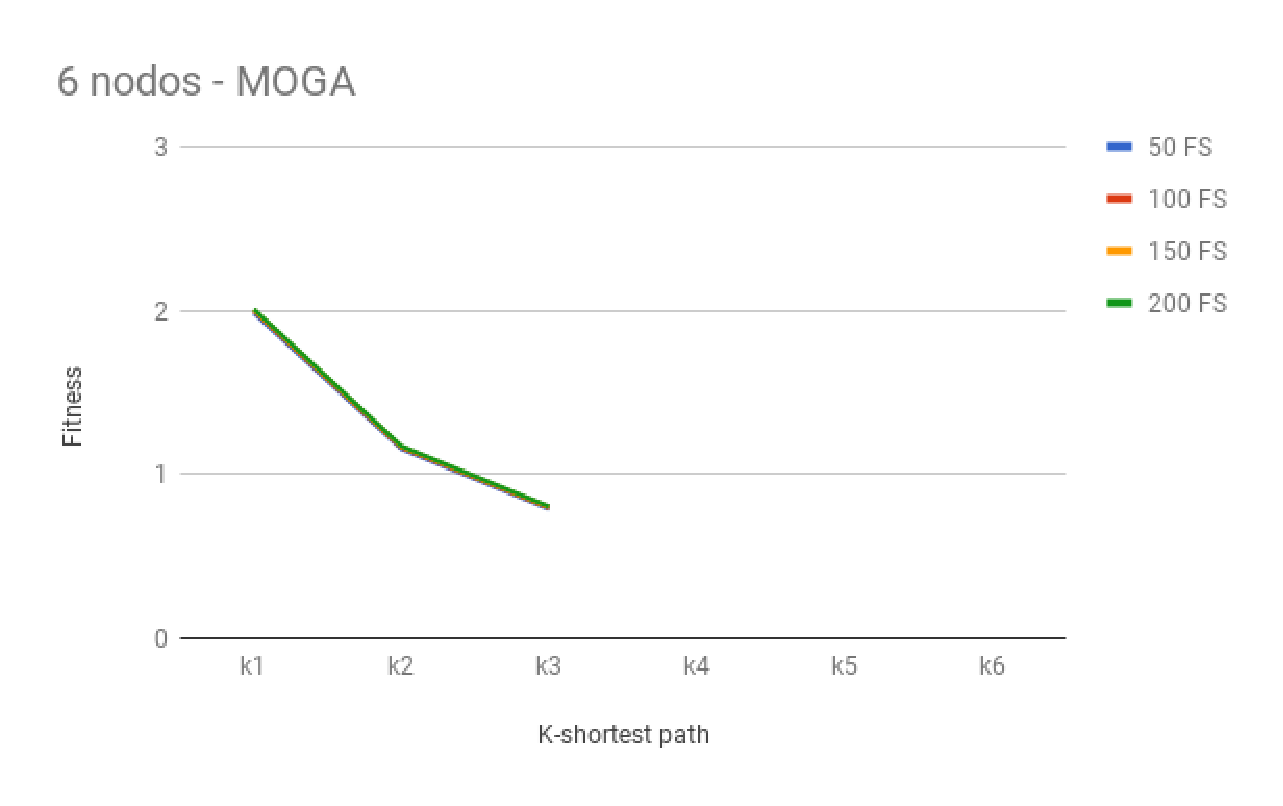
\includegraphics[scale=0.6]{G:/Genetico/LIBRO_TESIS/resulYsapy/resultados/6nodos_uniforme_moga1_fitness}
\par\end{centering}
\caption{Average fitness obtained by the MOGA talks topology of 6 nodes with
uniform charge}
\label{6nodos_moga1_fitness}
\end{figure}

\begin{figure}
\begin{centering}
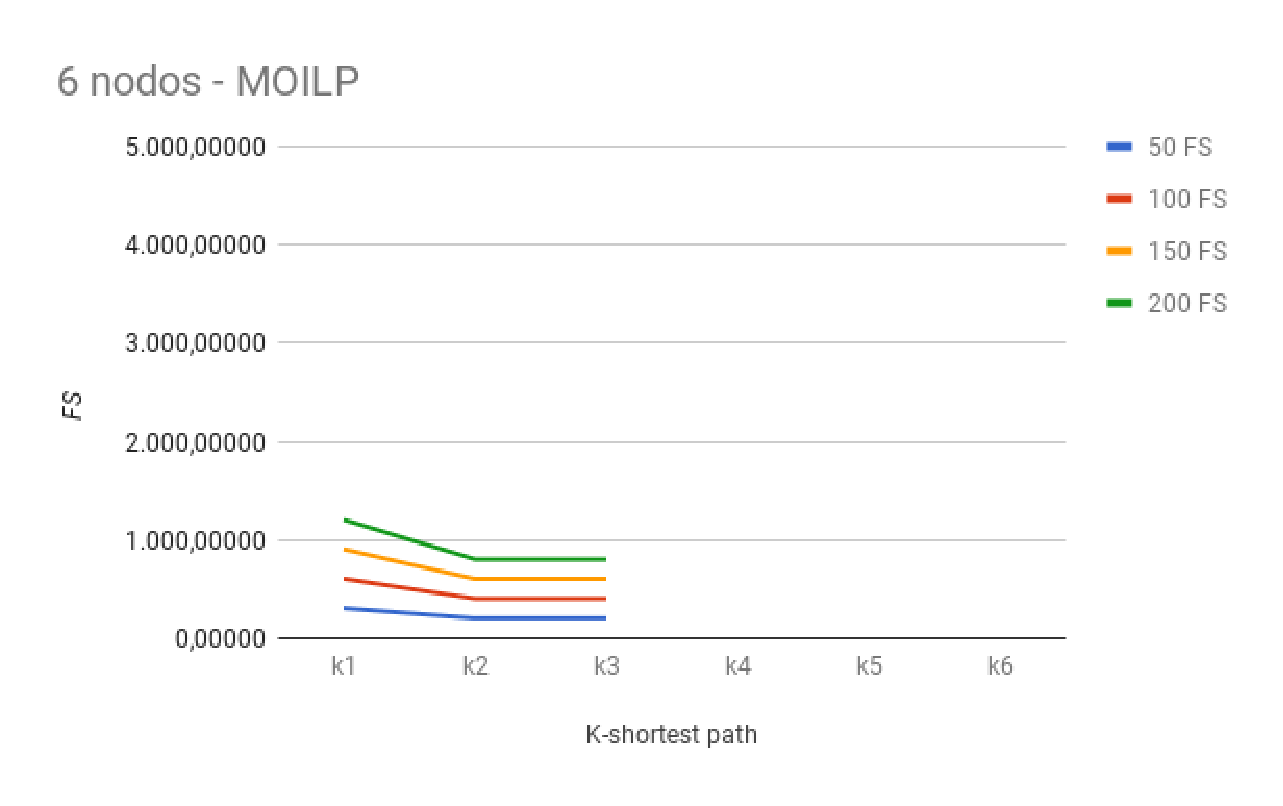
\includegraphics[scale=0.6]{G:/Genetico/LIBRO_TESIS/resulYsapy/resunif/6nodos_uniforme_ilp_fs}
\par\end{centering}
\caption{Maximum FS obtained by the MOILP for the topology of 6 nodes with
uniform load.}
\label{6nodos_ilp_fs}
\end{figure}

\begin{figure}
\begin{centering}
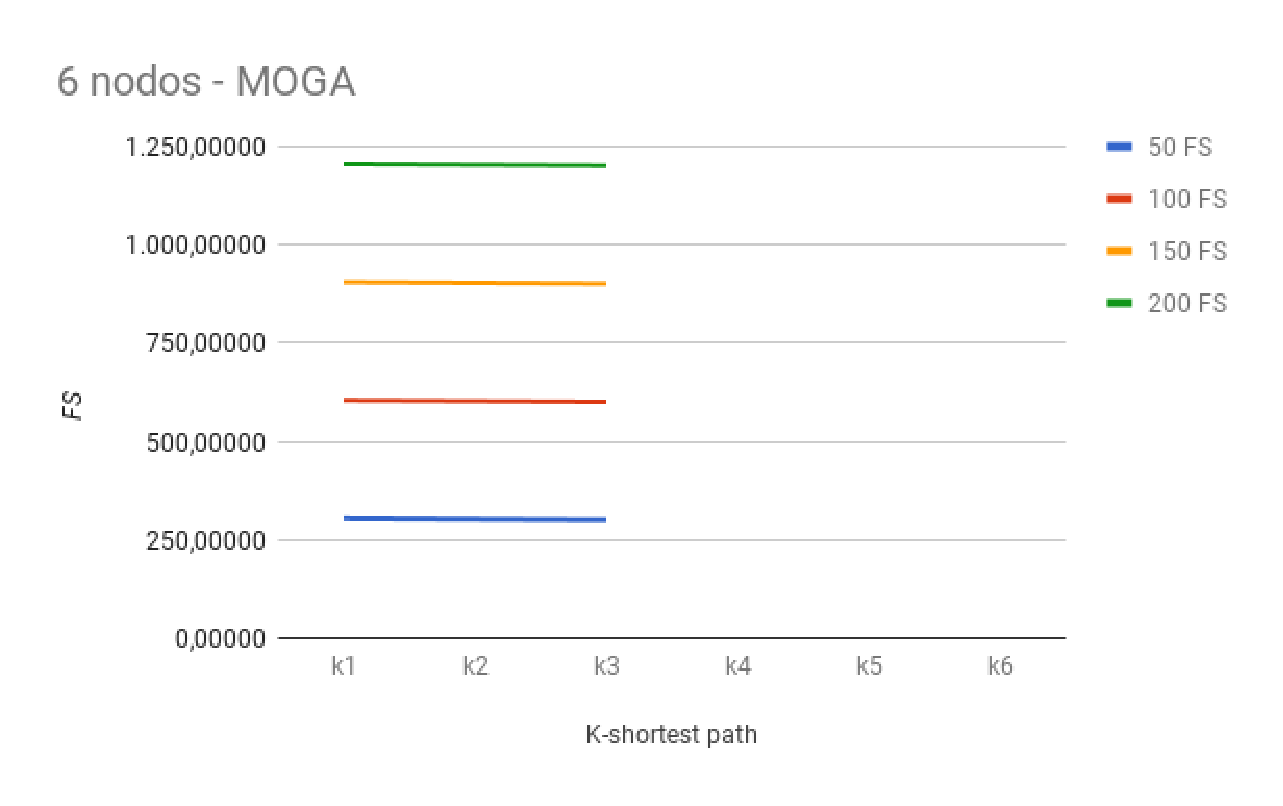
\includegraphics[scale=0.6]{G:/Genetico/LIBRO_TESIS/resulYsapy/resunif/6nodos_uniforme_moga1_fs}
\par\end{centering}
\caption{Maximum average FS obtained by the MOGA for the topology of 6 nodes
with uniform load.}
\label{6nodos_moga1_fs}
\end{figure}

\begin{figure}
\begin{centering}
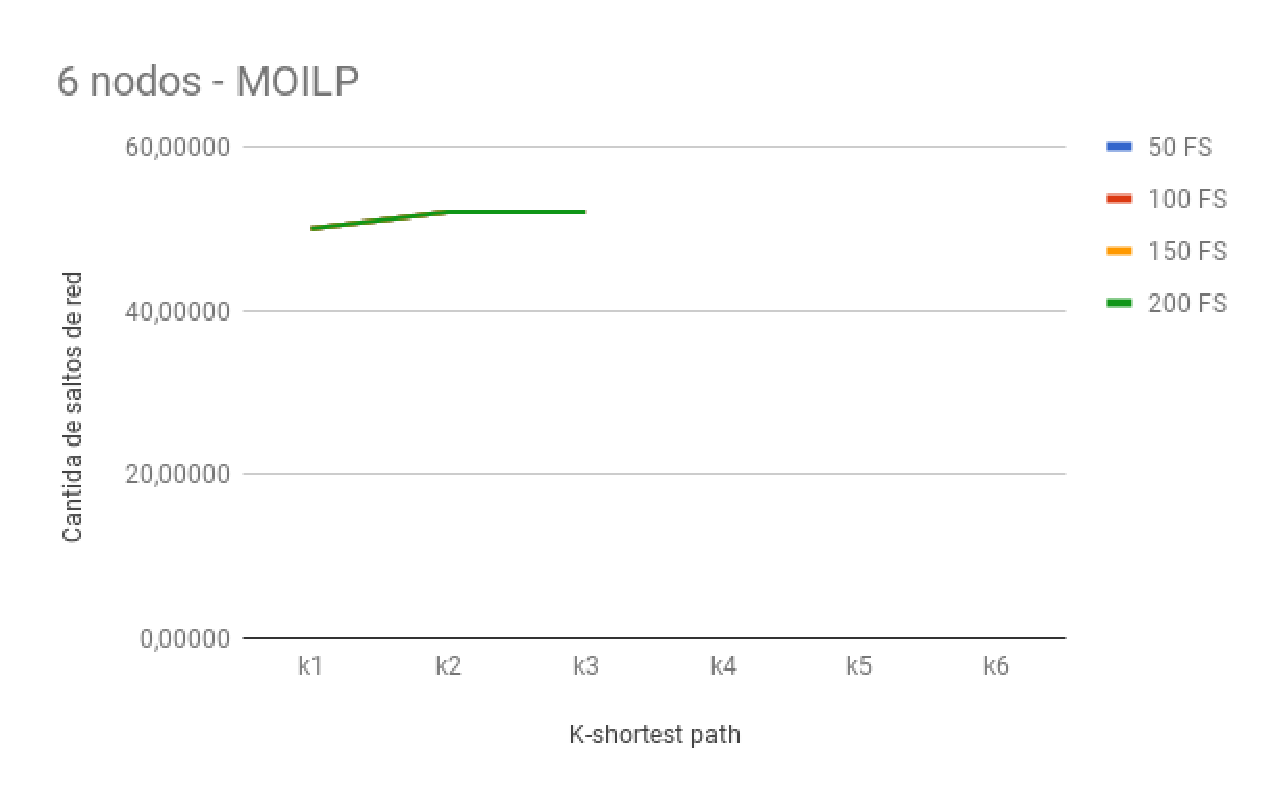
\includegraphics[scale=0.6]{G:/Genetico/LIBRO_TESIS/resulYsapy/resunif/6nodos_uniforme_ilp_distancia}
\par\end{centering}
\caption{Total distance obtained by the MOILP for the topology of 6 nodes with
uniform load.}
\label{6nodos_ilp_distance}
\end{figure}

\begin{figure}
\begin{centering}
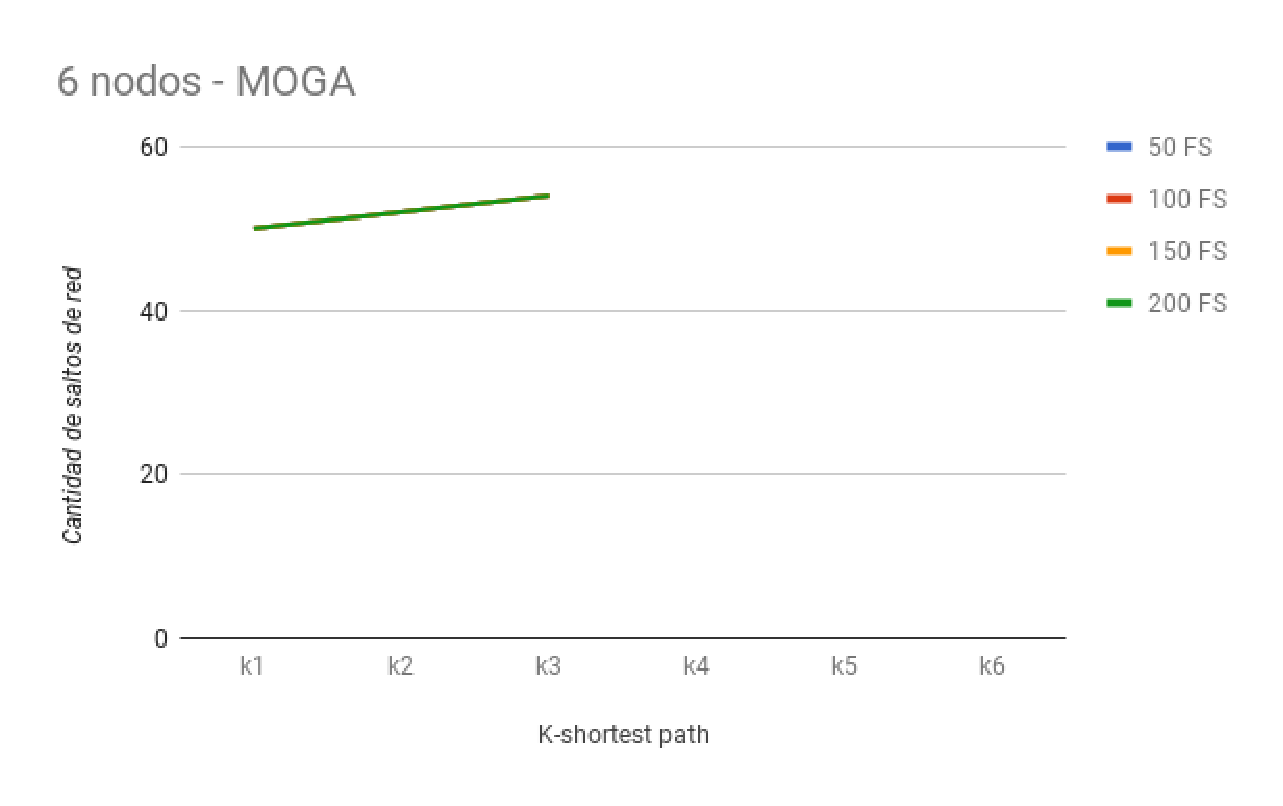
\includegraphics[scale=0.6]{G:/Genetico/LIBRO_TESIS/resulYsapy/resunif/6nodos_uniforme_moga1_distancia}
\par\end{centering}
\caption{Average total distance obtained by the MOGA for the topology of 6
nodes with uniform load}
\label{6nodos_moga1_distance}
\end{figure}

\begin{figure}
\begin{centering}
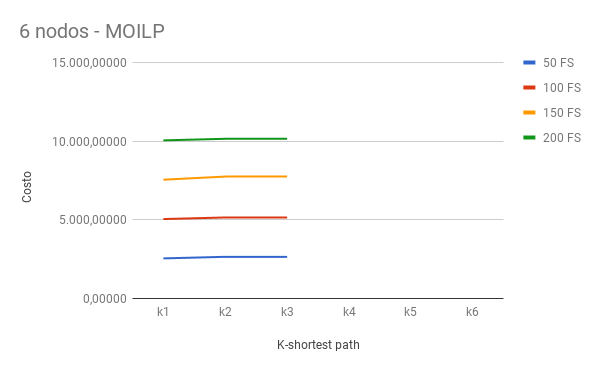
\includegraphics[scale=0.6]{G:/Genetico/LIBRO_TESIS/resulYsapy/resunif/6nodos_uniforme_ilp_costo}
\par\end{centering}
\caption{Total cost obtained by MOILP for the topology of 6 nodes with uniform
load.}
\label{6nodos_ilp_cost}
\end{figure}

\begin{figure}
\begin{centering}
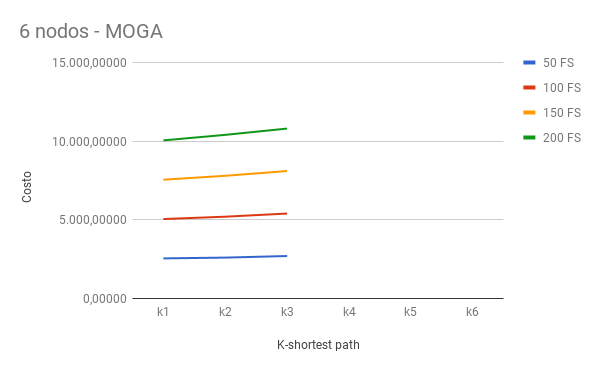
\includegraphics[scale=0.6]{G:/Genetico/LIBRO_TESIS/resulYsapy/resunif/6nodos_uniforme_moga1_costo}
\par\end{centering}
\caption{Average total cost obtained by the MOGA for the topology 6 nodes with
uniform load.}
\label{6nodos_moga1_cost}
\end{figure}

\begin{figure}
\begin{centering}
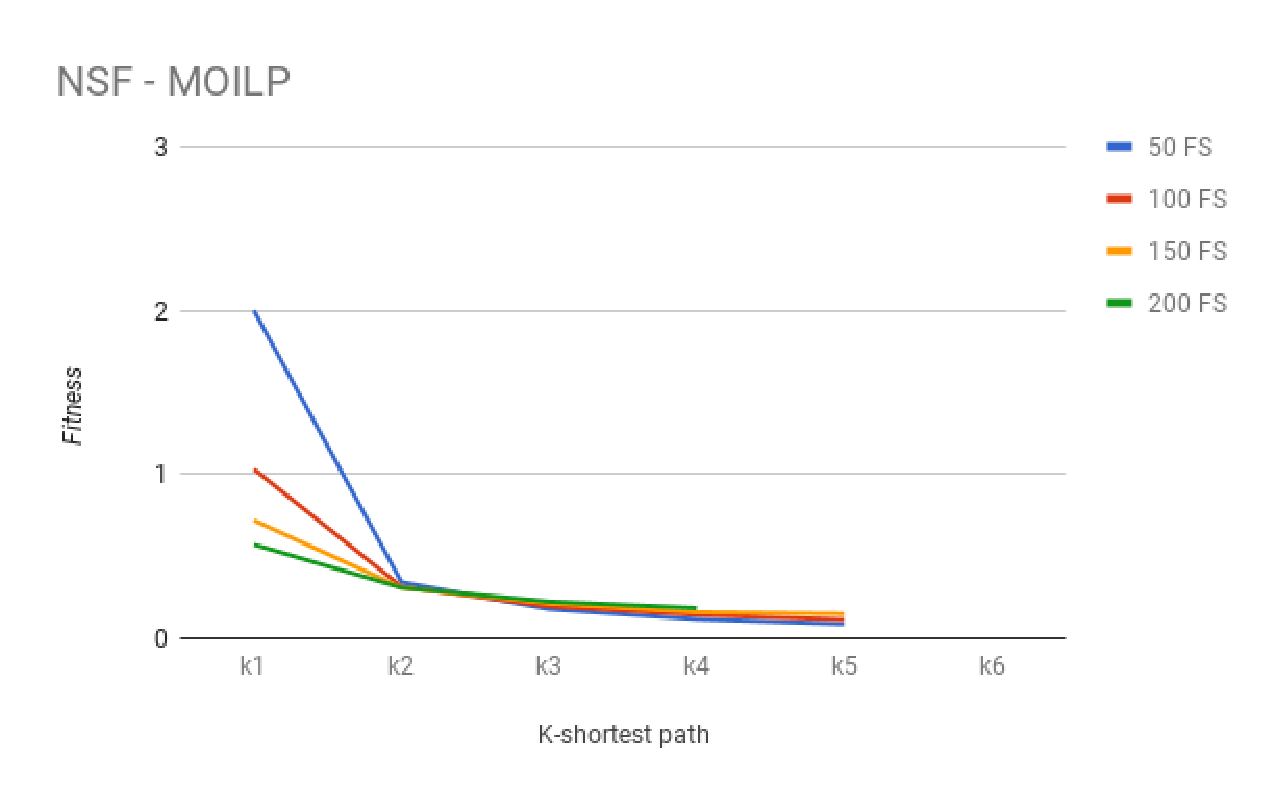
\includegraphics[scale=0.6]{G:/Genetico/LIBRO_TESIS/resulYsapy/resultados/nsf_uniforme_ilp_fitness}
\par\end{centering}
\caption{Fitness obtained by MOILP for topology NSF-14 with uniform load.}
\label{nsf-14_ilp_fitness}
\end{figure}

\begin{figure}
\begin{centering}
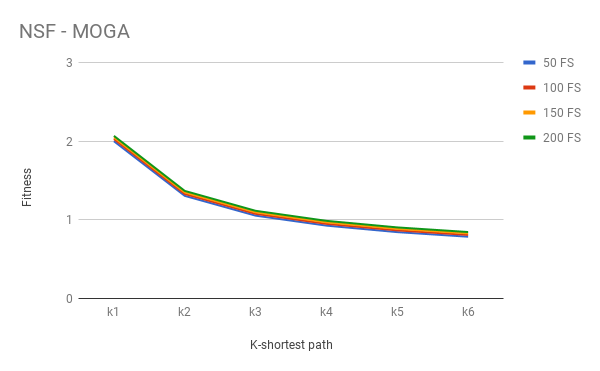
\includegraphics[scale=0.6]{G:/Genetico/LIBRO_TESIS/resulYsapy/resultados/nsf_uniforme_moga1_fitness}
\par\end{centering}
\caption{Average fitness obtained by the MOGA talks topology of NSF-14 with
uniform charge}
\label{nsf-14_moga1_fitness}
\end{figure}

\begin{figure}
\begin{centering}
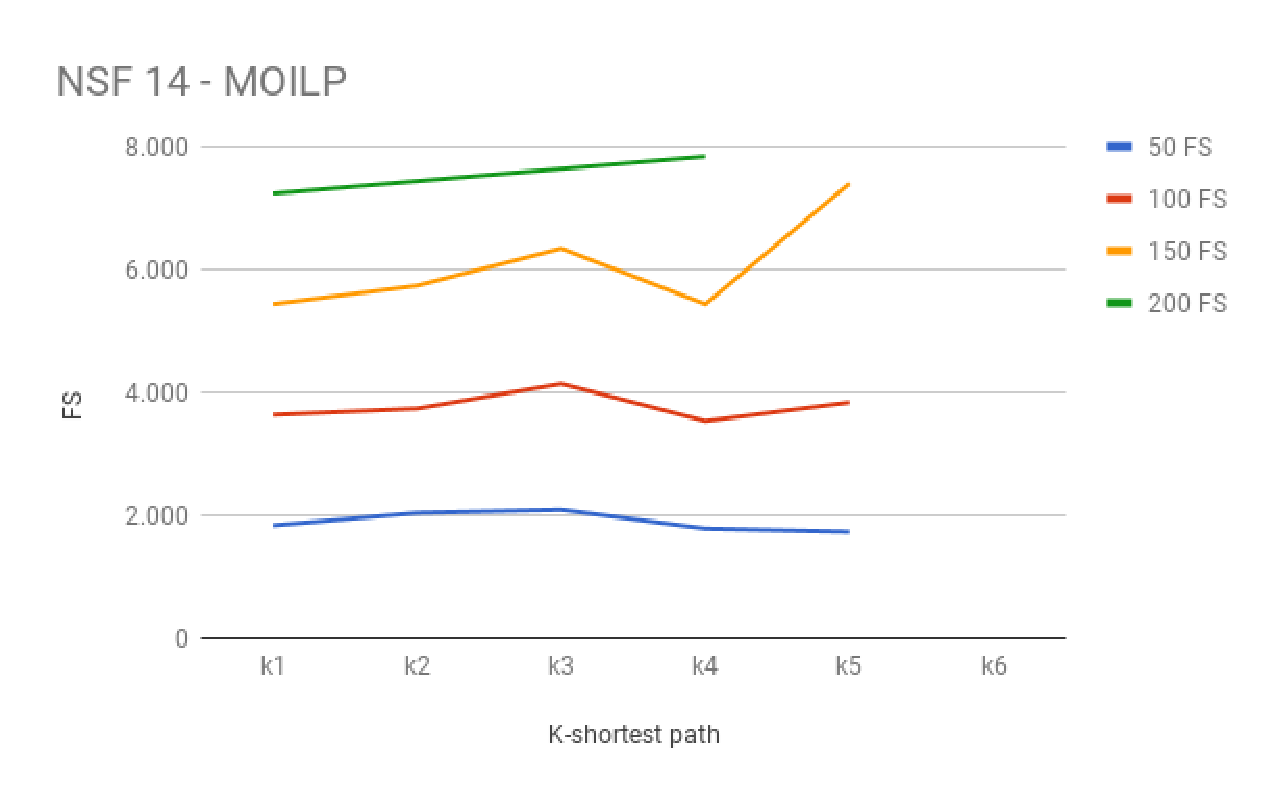
\includegraphics[scale=0.6]{G:/Genetico/LIBRO_TESIS/resulYsapy/resunif/nsf_uniforme_ilp_fs}
\par\end{centering}
\caption{Maximum FS obtained by the MOILP for the topology of NSF-14 with uniform
load.}
\label{nsf-14_ilp_fs}
\end{figure}

\begin{figure}
\begin{centering}
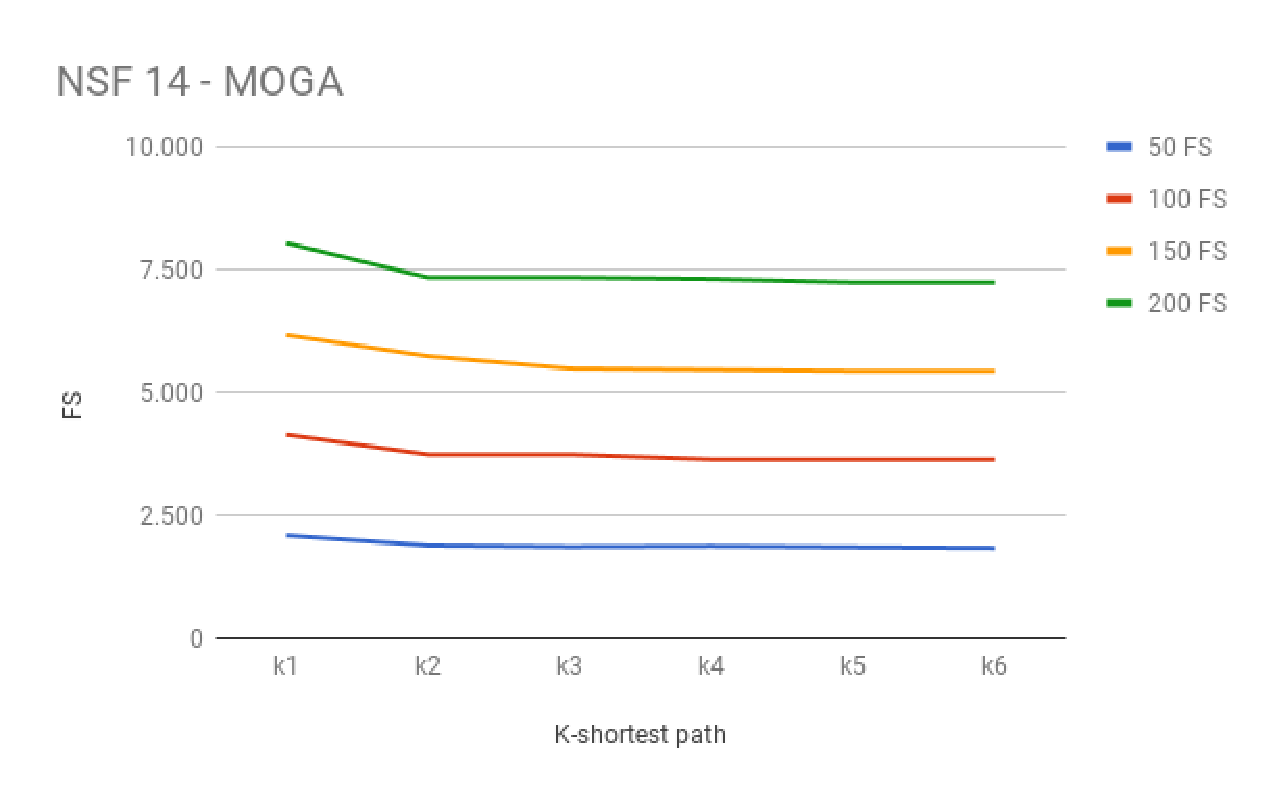
\includegraphics[scale=0.6]{G:/Genetico/LIBRO_TESIS/resulYsapy/resunif/nsf_uniforme_moga1_fs}
\par\end{centering}
\caption{Maximum average FS obtained by the MOGA for the topology of NSF-14
with uniform load.}
\label{nsf-14_moga1_fs}
\end{figure}

\begin{figure}
\begin{centering}
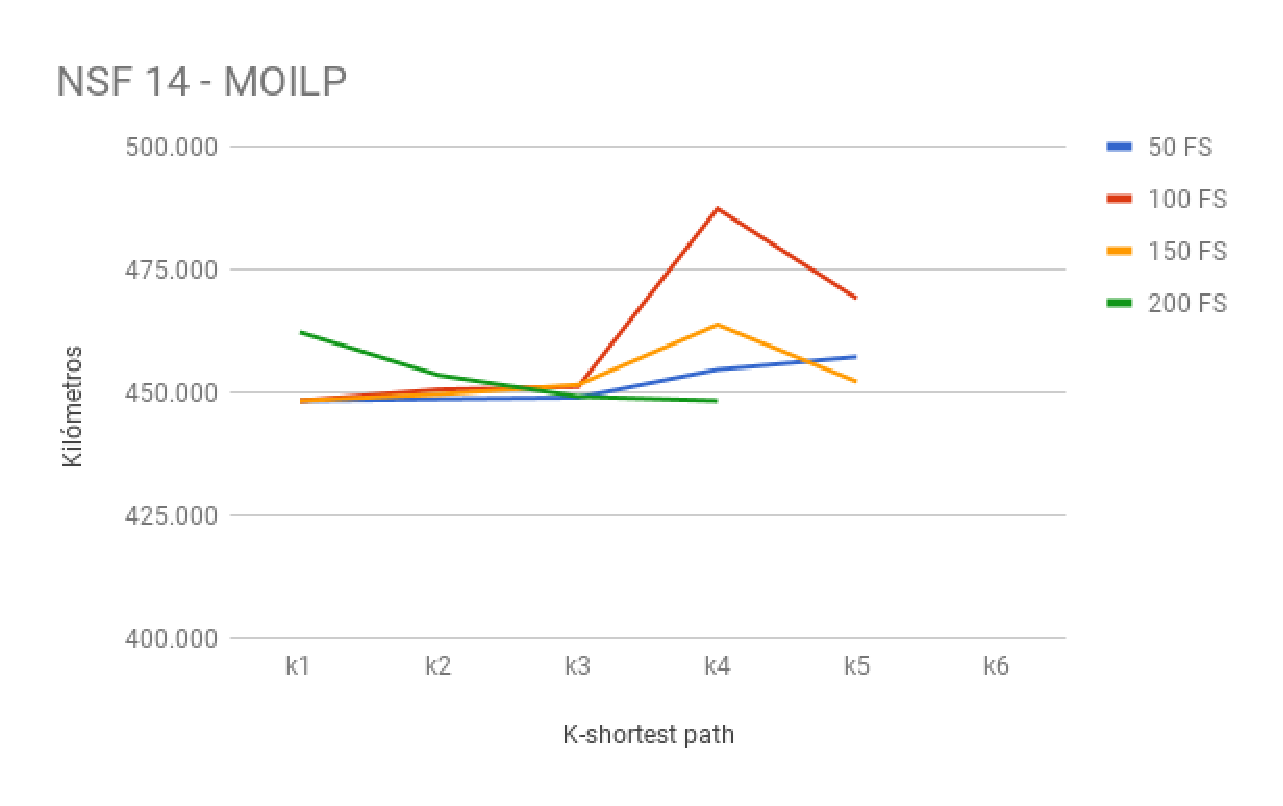
\includegraphics[scale=0.6]{G:/Genetico/LIBRO_TESIS/resulYsapy/resunif/nsf_uniforme_ilp_distancia}
\par\end{centering}
\caption{Total distance obtained by the MOILP for the topology of NSF-14 with
uniform load.}
\label{nsf-14_ilp_distance}
\end{figure}

\begin{figure}
\begin{centering}
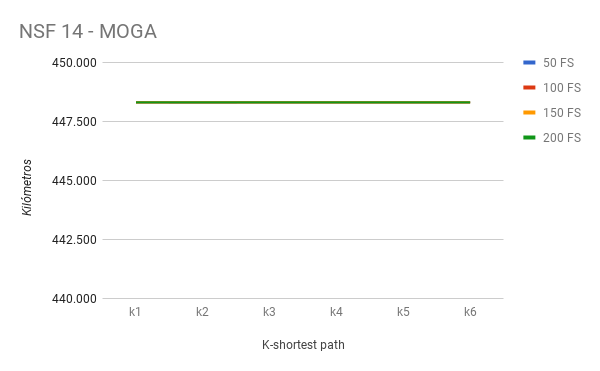
\includegraphics[scale=0.6]{G:/Genetico/LIBRO_TESIS/resulYsapy/resunif/nsf_uniforme_moga1_distancia}
\par\end{centering}
\caption{Average total distance obtained by the MOGA for the topology of NSF-14
with uniform load}
\label{nsf-14_moga1_distance}
\end{figure}

\begin{figure}
\begin{centering}
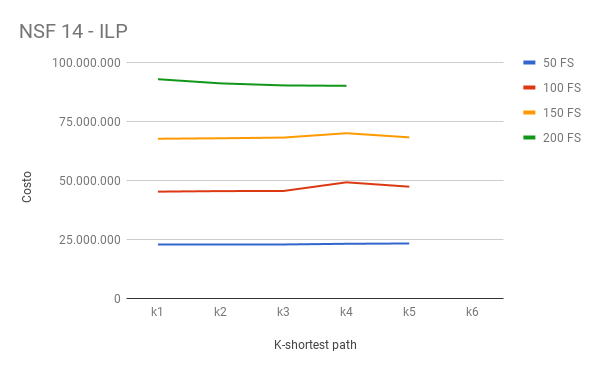
\includegraphics[scale=0.6]{G:/Genetico/LIBRO_TESIS/resulYsapy/resunif/nsf_uniforme_ilp_costo}
\par\end{centering}
\caption{Total cost obtained by MOILP for the topology of NSF-14 with uniform
load.}
\label{nsf-14_ilp_cost}
\end{figure}

\begin{figure}
\begin{centering}
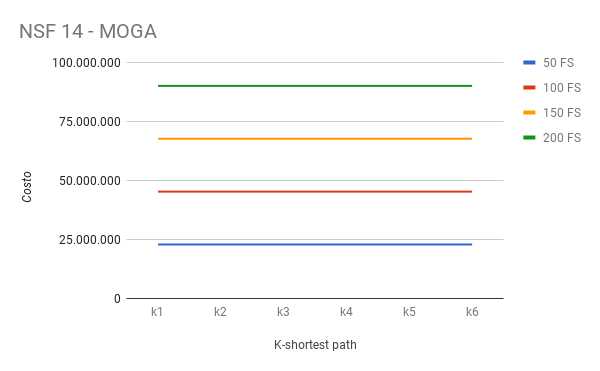
\includegraphics[scale=0.6]{G:/Genetico/LIBRO_TESIS/resulYsapy/resunif/nsf_uniforme_moga1_costo}
\par\end{centering}
\caption{Average total cost obtained by the MOGA for the topology NSF-14 with
uniform load.}
\label{nsf-14_moga1_cost}
\end{figure}

\begin{figure}
\begin{centering}
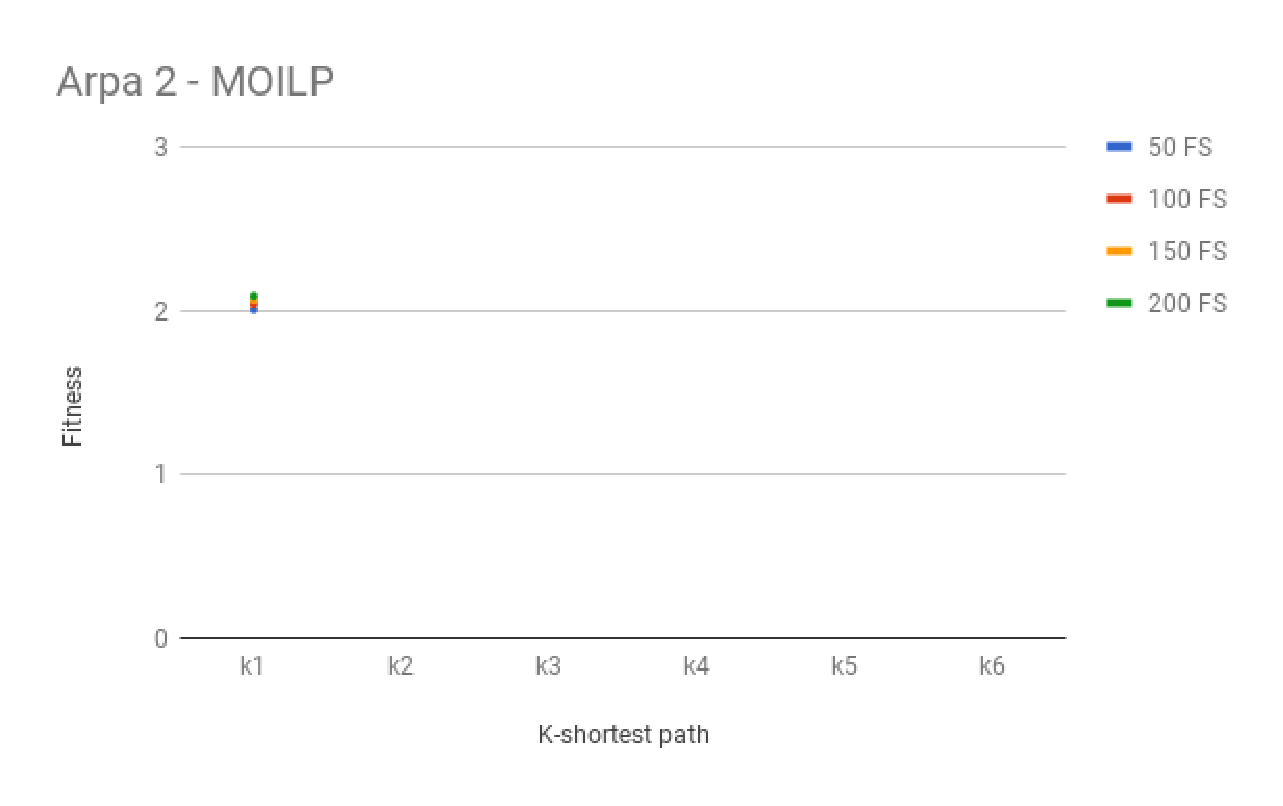
\includegraphics[scale=0.6]{G:/Genetico/LIBRO_TESIS/resulYsapy/resultados/arpa_uniforme_ilp_fitness}
\par\end{centering}
\caption{Fitness obtained by MOILP for topology ARPA-2 with uniform load.}
\label{arpa-2_ilp_fitness}
\end{figure}

\begin{figure}
\begin{centering}
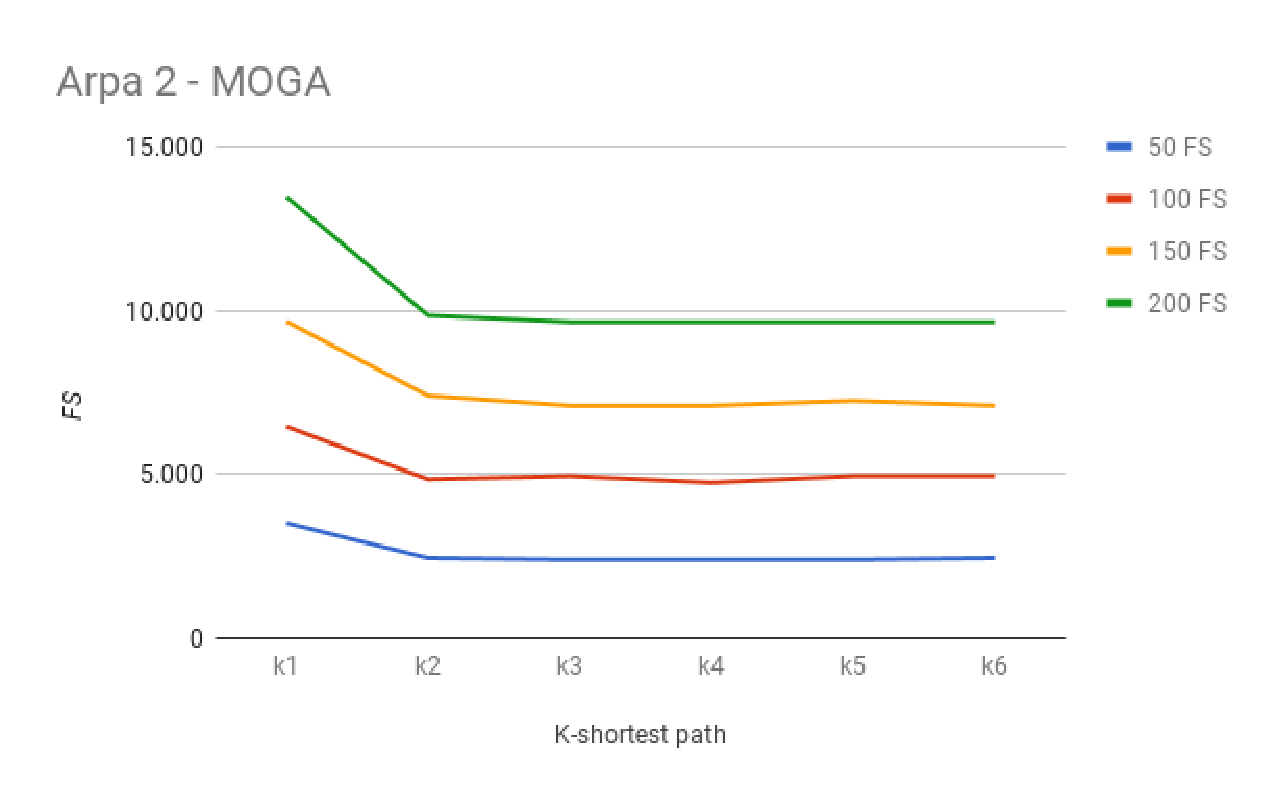
\includegraphics[scale=0.6]{G:/Genetico/LIBRO_TESIS/resulYsapy/resunif/arpa_uniforme_moga1_fs}
\par\end{centering}
\caption{Maximum average FS obtained by the MOGA talks topology of ARPA-2 with
uniform charge}
\label{arpa-2_moga1_fs}
\end{figure}

\begin{figure}
\begin{centering}
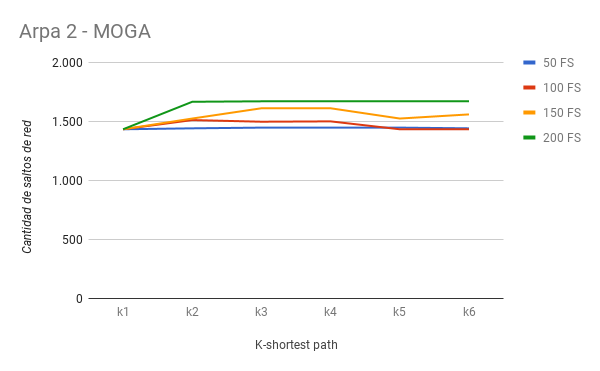
\includegraphics[scale=0.6]{G:/Genetico/LIBRO_TESIS/resulYsapy/resunif/arpa_uniforme_moga1_distancia}
\par\end{centering}
\caption{Total distance obtained by the MOGA for the topology of ARPA-2 with
uniform load.}
\label{arpa-2_moga1_distance}
\end{figure}

\begin{figure}
\begin{centering}
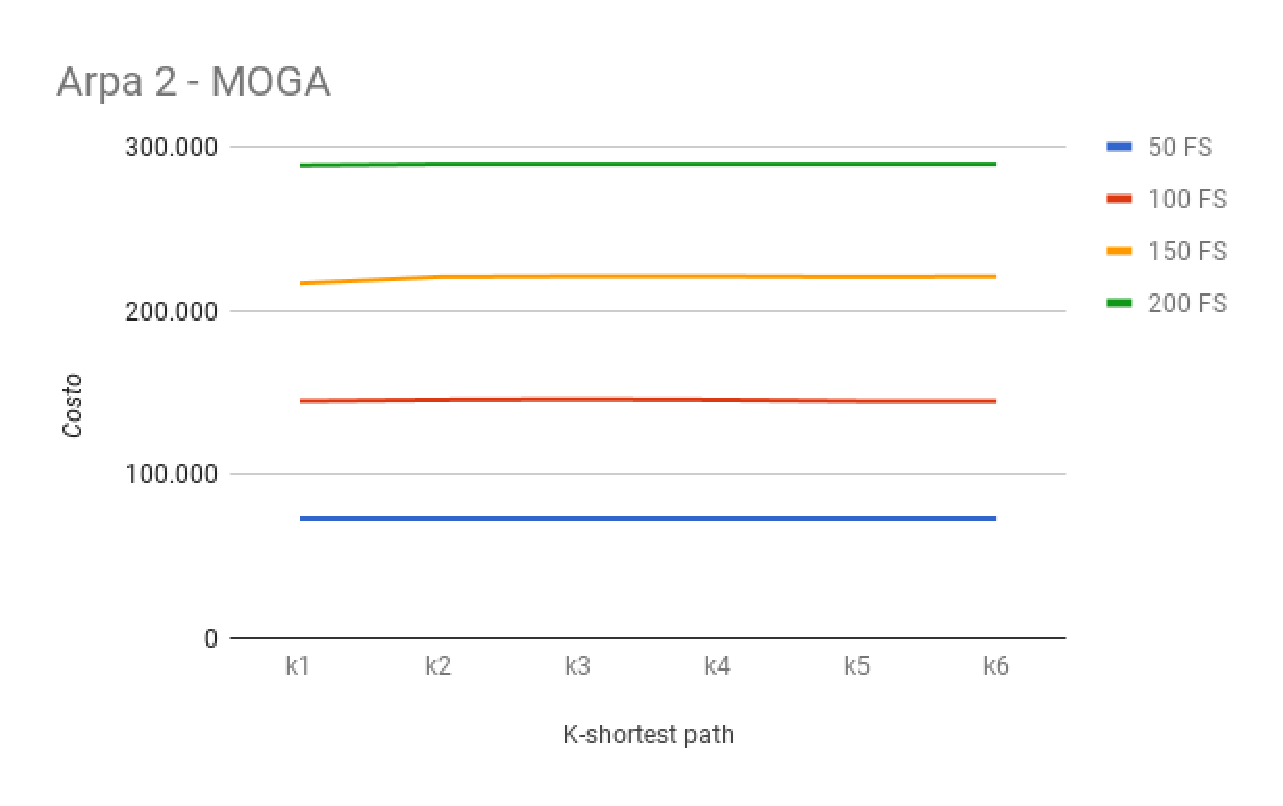
\includegraphics[scale=0.6]{G:/Genetico/LIBRO_TESIS/resulYsapy/resunif/arpa_uniforme_moga1_costo}
\par\end{centering}
\caption{Average total cost obtained by the MOGA for the topology of ARPA-2
with uniform load.}
\label{arpa-2_moga1_cost}
\end{figure}


\section{NSGAII{*} vs NSGS II}

In this section we present the difference with the work proposed in
\cite{moga-rsa-dao} and the work presented by us, in addition the
results of the experimental tests are presented and analyzed. The
work proposed in \cite{moga-rsa-dao}, presents the multi-objective
RSA problem and its associated algorithm model. Each request has many
possible routes, and in each routing it has several spectrum assignment
options. The problem is to minimize the spectrum width to support
all requests and minimize the overall cost of the spectrum in the
link. 

The objective function for the work proposed in \cite{moga-rsa-dao}
is as follows: there are two objectives associated with each chromosome.
The first objective $f_{1}$, is the width of the spectrum that indicates
the maximum indexed slice used in the network. The second objective
$f_{2}$ is the total cost of the spectrum link. Given a chromosome,
the route and channel are calculated for each demand. After attending
each demand sequentially and without any sort of ordering, the spectrum
availabilities vector of each link is updated. 

In this developed work, which is an extension of the work presented
in \cite{engopt} which has an approach based on weighted sum, a pure
multi-objective approach with Pareto fronts is presented. In our work,
as in \cite{moga-rsa-dao} it has many possible routes, and in each
routing it has several spectrum assignment options. The problem is
to minimize the spectrum width to support all requests and minimize
the overall cost of the link spectrum. The same objective function
is taken from \cite{moga-rsa-dao} and the requests are handled as
follows: applications are ordered from highest to lowest, defined
by the highest possible cost of said request, the first 30\% of said
list is attended in the first place, while the remaining 70\% is treated
in a random manner, unlike \cite{moga-rsa-dao} it is a random ordering. 

The tests carried out considering different types of traffic load,
on the NSF topology (Figure \ref{topology_nsf_figure}), different
K values (paths) and different amounts of demands, try to replicate
various possible scenarios of the problem to solve. The experimental
tests carried out show that our proposal for the ordering of the requests
presents promising results. 

\subsection{Testing environment }

The experiments were performed on a computer with an Intel Core i3
processor (3.40 GHz) and 8 GB of RAM. The implementation and execution
of the MOEAs were carried out with JAVA 8. 

The traffic loads used were of the all-to-all type, that is, each
node of the network makes a transfer request to all others in the
network. In addition, the type of traffic load was random. The loads
are divided into 3 categories, 50, 100 and 150 (low, medium, high),
that is to say that for the category of 50 FS, for each demand a random
value between 1 and 50 was generated as a requested quantity of FS;
For category 100, for each demand a random value between 1 and 100
was generated as the requested quantity of FS and for category 150,
a random value of 1 and 150 was generated as requested quantity of
FS. Another variant that was taken into account for the execution
of the tests was the number of shortest routes pre-calculated, that
is, the value K. They were made with the following values of k = 2,
3, 4 and 5 for the network. For the executions of the NSGA II, the
values shown in Table 1 were used as evolutionary parameters. The
metric used for the comparison of the algorithms are hyper-volume
and coverage \cite{engopt}. 

Based on these steps, the experimental results are presented.

\begin{table}
\caption{Parameters used for the execution of the MOEA's}

\centering{}%
\begin{tabular}{cc}
\hline 
\textbf{Parameters} & \textbf{Value}\tabularnewline
\hline 
Size of the population & 50\tabularnewline
\hline 
Probability of mutation & 0.1\tabularnewline
\hline 
Stop Criterion (in minutes) & 5\tabularnewline
\hline 
Number of independent runs & 15\tabularnewline
\hline 
\end{tabular}
\end{table}


\subsection{Hyper-volume Metric }

For the hyper-volume metric you can see the table number 2, for load
type 50 (low), with the number of paths k = 2, our proposed algorithm
of order 30/70 obtains better results before the algorithm without
ordering. For load type 50 (low), with k = 3 paths, again our algorithm
with order 30/70, exceeds the algorithm without ordering. For load
type 50 with k = 4, the algorithm without ordering obtained better
results with our algorithm 30/70. For k = 5 with 50 loading (low),
our algorithm 30/70 obtained good results. For k = 2 with 100 load
(average), the algorithm without ordering obtained better results,
k = 3 with 100 load (average), our algorithm with order 30/70, has
better results before the algorithm without ordering, for k = 4 with
100 load (average), our 30/70 sorting algorithm improves the results
before the algorithm without ordering. For k = 5 with 100 of load
(average), we obtained very good results with respect to the algorithm
without ordination. 

For k = 2 with 150 loading (high), our sort algorithm 30/70 obtained
better results compared to the algorithm without ordering. In k =
3 with 150 loading (high), the algorithm without ordination obtained
good results. Our 30/70 sorting algorithm got better results when
k = 4 with 150 loading (high) compared to the unordered algorithm.
The unordered algorithm had better results when k = 5 and the load
is 150 (high), compared to our 30/70 sorting algorithm.

\subsection{Coverage Metric }

For the coverage metric we analyze the table number 3, where it can
be seen when the load type is 50 (low) and the number of roads k =
2, our ordering algorithm 30/70 obtained a greater coverage before
the algorithm without ordination. For k = 3 with 50 load (low), our
algorithm obtained a greater coverage with respect to the algorithm
without ordering. For when k = 4 and 50 of load (low), the algorithm
without ordination obtained a greater coverage before our algorithm
of ordering 30/70. With k = 5 and the load of 50 (low), our ordering
algorithm 30/70 obtained a better coverage. For load type 100 (average)
with k = 2, the unordered algorithm had better coverage in our ordering
algorithm 30/70. When k = 3 with load type 100 (average), our algorithm
obtained better coverage before the algorithm without ordering. With
a load of 100 (average) and k = 4, our algorithm obtained better coverage
than the algorithm without ordination. When k = 5 and load type 100
(average), our algorithm obtained better coverage than the algorithm
without ordination. 

For load type 150 (high) with k = 2, our algorithm showed better coverage
than the algorithm without ordination, for k = 3 and 150 load (high),
the algorithm without ordination yielded better coverage than our
ordering algorithm. 30/ 70 For k = 4 with 150 loading (high), our
algorithm obtained better coverage before the algorithm without ordering.
For k = 4 with a load of 150 (high), the algorithm without ordering
obtained better coverage. For k = 5 with 150 loading (high), our algorithm
obtained better coverage than the non-ordered algorithm. 
\begin{center}
\begin{table}
\caption{Comparision of algorithms, hyper-volumen metric}

\centering{}%
\begin{tabular}{|>{\raggedright}m{2cm}|>{\centering}m{2cm}|l|l|}
\hline 
\centering{}\textbf{Type of load (low, mid, high)} & \textbf{Number of roads (k)} & \textbf{Sorting Algorithm 30/70} & \textbf{Unsorted Algorithm}\tabularnewline
\hline 
\hline 
\multirow{4}{2cm}{\centering{}50} & 2 & \textbf{0,00450575727952277000} & 0,00373184833987698000\tabularnewline
\cline{2-4} 
 & 3 & \textbf{0,03004763727709010000} & 0,00114619949446014000\tabularnewline
\cline{2-4} 
 & 4 & 0,00107277586229790000 & \textbf{0,00608913898555240000}\tabularnewline
\cline{2-4} 
 & 5 & \textbf{0,01524133420666540000} & 0,01404235292493280000\tabularnewline
\hline 
\multirow{4}{2cm}{\centering{}100} & 2 & 0,00000000040137206552 & \textbf{0,00000000428130203222}\tabularnewline
\cline{2-4} 
 & 3 & \textbf{0,00235590742252450000} & 0,00192187663358532000\tabularnewline
\cline{2-4} 
 & 4 & \textbf{0,00000000625575249301} & 0,00000000039930335062\tabularnewline
\cline{2-4} 
 & 5 & \textbf{0,00000000560063877525} & 0,00000000040004562680\tabularnewline
\hline 
\multirow{4}{2cm}{\centering{}150} & 2 & \textbf{0,00000000437845029918} & 0,00000000027365314370\tabularnewline
\cline{2-4} 
 & 3 & 0,00004759974150804820 & \textbf{0,00063478877339381300}\tabularnewline
\cline{2-4} 
 & 4 & \textbf{0,00036203376622539800} & 0,00003620284610853910\tabularnewline
\cline{2-4} 
 & 5 & 0,00004690367773651360 & \textbf{0,00171967667778795000}\tabularnewline
\hline 
\end{tabular}
\end{table}
\par\end{center}

\begin{center}
\begin{table}
\caption{Comparision of algorithms, coverage metric}

\centering{}%
\begin{tabular}{|>{\centering}m{2cm}|>{\centering}m{2cm}|c|c|}
\hline 
\textbf{Type of load (low, mid, high)} & \textbf{Number of roads (k)} & \textbf{Sorting Algorithm 30/70} & \textbf{Unsorted Algorithm}\tabularnewline
\hline 
\hline 
\multirow{4}{2cm}{\centering{}50} & 2 & \textbf{0,6} & 0,3\tabularnewline
\cline{2-4} 
 & 3 & \textbf{1,0} & 0,0\tabularnewline
\cline{2-4} 
 & 4 & 0,0 & \textbf{1,0}\tabularnewline
\cline{2-4} 
 & 5 & \textbf{0,5} & 0,0\tabularnewline
\hline 
\multirow{4}{2cm}{\centering{}100} & 2 & 0,0 & \textbf{1,0}\tabularnewline
\cline{2-4} 
 & 3 & \textbf{0,3} & 0,0\tabularnewline
\cline{2-4} 
 & 4 & \textbf{1,0} & 0,0\tabularnewline
\cline{2-4} 
 & 5 & \textbf{1,0} & 0,0\tabularnewline
\hline 
\multirow{4}{2cm}{\centering{}150} & 2 & \textbf{1,0} & 0,0\tabularnewline
\cline{2-4} 
 & 3 & 0,0 & \textbf{1,0}\tabularnewline
\cline{2-4} 
 & 4 & \textbf{1,0} & 0,0\tabularnewline
\cline{2-4} 
 & 5 & 0,0 & \textbf{1,0}\tabularnewline
\hline 
\end{tabular}
\end{table}
\par\end{center}
